\documentclass{book}
\usepackage{tikz,xcolor}
\author{Martin}
\date{\today}

\begin{document}
\maketitle

    \begin{center}
        \begin{tikzpicture}
            \draw[thick](0,0) -- (3,3);
            \draw[thin](0,0) -- (3,-3);
            \draw[very thin](0,0) -- (-3,-3);
            \draw[ultra thick] (0,0) -- (-3,3);
        \end{tikzpicture}

        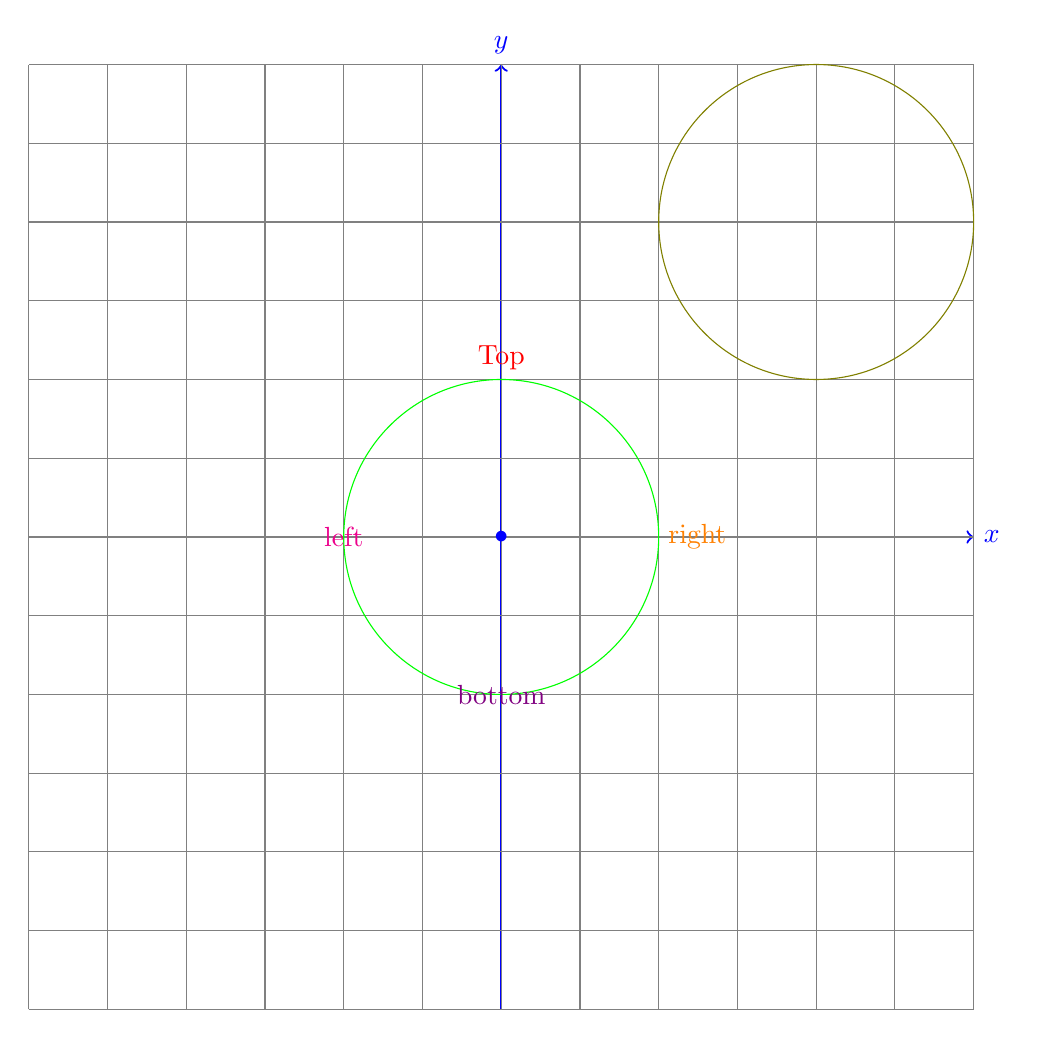
\begin{tikzpicture}[scale=2]
            \draw[thick,blue,->](0,-3)--(0,3) node[above] {$y$};
            \draw[thick,blue,->](-3,0)--(3,0) node[right] {$x$};
            \draw[color=gray,thin,step=0.5] (-3,-3) grid (3,3);
            \draw[color=green, thin] (0,0) circle (1cm);
            \node[blue] at (0,0) {\(\bullet\)};
            \node[red,above] at (0,1) {Top};
            \node[orange,right] at (1,0) {right};
            \node[magenta] at (-1,0) {left};
            \node[violet] at (0,-1) {bottom};
            \draw[color=green!50!red] (2,2) ellipse (1cm and 1cm);
        \end{tikzpicture}
    \end{center}

\end{document}
